\chapter{Introduction} \label{intro}

Weather related natural disaster cost the world economy around 100 billion dollars every year \citep{Kousky2014}. The \citet{CRED2015} calculated that an average of 69.800 deaths per year are inflicted due to these disasters, combined with earthquakes. The effects are felt around the world,  however most deaths occur in low or middle income areas. The interval between disasters is shortening, resulting in more disaster per year [figure \ref{fig:graph1}]. They are furthermore causing more damage than before, with the most economic damage in 2011 \citep{Kerle2015}. 2017 was an exceptional year, less people were killed by natural disasters, however the economic damages where much larger than average \citep{RE2018}. 
\\
\begin{figure}[h]
	\centering
	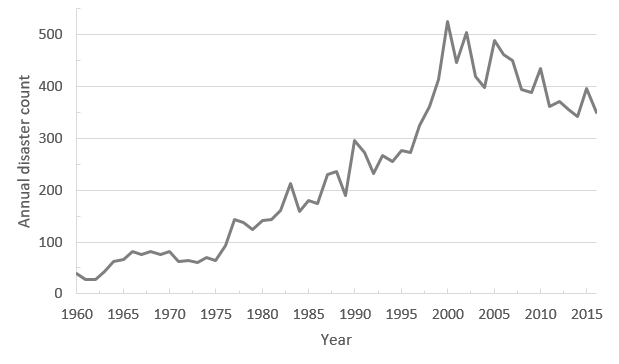
\includegraphics[width=0.9\textwidth]{figs/graph2.png}
	\caption{Natural disaster per year from 1960 to 2016 [From:  EM-DAT: The Emergency Events Database - Universite catholique de Louvain (UCL) - CRED, D. Guha-Sapir - www.emdat.be, Brussels, Belgium]}
	\label{fig:graph1}
\end{figure}

\section{Hurricane Irma}
One of the major disasters of 2017 was hurricane Irma, being labelled the worst storm in the Caribbean in recorded history \citep{Daniell2017}. In the first week of September this hurricane raged over multiple islands causing billions worth of damage, affecting millions in its path \citep{Phipps2017,Daniell2017}. One of the islands affected is St. Maarten, part of the Kingdom of the Netherlands. It was hit by the eye of the hurricane on the 6th of September with winds up to 185 miles per hour \citep{Wilts2017}. Two other major hurricane passed over the area in the weeks following hurricane Irma, however, fortunately these did little to no extra damage on the island \citep{Gray2017,Bijnsdorp2017}. First damage estimates show that 70 - 90\% of the island may be affected by the storm \citep{Rodekruis2017,UNOSAT2017}. The indication and location of the damage caused is a leading planning tool for organisations like the \ac{nlrc}, providing a first indication of the most vulnerable people in an affected area. Indications of damage have allowed the \ac{nlrc} to help 18.881 individual people since the landfall of hurricane Irma and subsequent relief operation; and long term operations are being started right now to facilitate the rebuilding of the island \citep{Rodekruis2017}. 
\\

\section{Remote Sensing}
In the context of disasters the decision making process and risk management process, as performed by the \ac{nlrc} are bounded by three key characteristics \citep{Zlatanova2008}. [1.] Rapid action needs to be taken, [2.] aware of the situation and context [3.] with a connected overview of the data available. The goal of the \ac{drm} is to minimize the impact from a disaster \citep{Piero2012}. Information on the extent of the damage is therefore paramount, as demonstrated by the relief operation from the \ac{nlrc}. Building damage is an essential indicator for this \citep{Schweier2006}; but can be hard to establish as it requires a lot of manual labour \citep{Kerle2010}. Automated detection of building damages could be the solution \citep{Vetrivel2016b}. \\
Remote sensing has long been part of the \ac{drm} cycle. According to \citet{Kerle2015} this started at the beginning of space-based remote sensing around the 1960s and 1970s and brought about the increase in information within the \ac{drm}. From here the development of remote sensing techniques accelerated over the past 50 years and increasingly allow for higher resolution information in a more timely manner. The performance increase in remote sensing solutions make it applicable for the automated classification of building damage \citep{DellAcqua2012,Dong2013}. Many solutions for automated damage detection or classification have been developed over the past years based on several remote sensing techniques. \citet{Dong2013} provides a clear overview of the solutions up until 2013 and several more have been developed since \citep{Dominici2017,Sharma2017,Kakooei2017,Vetrivel2016b,Menderes2015}. However in practice service from the International Charter, like Copernicus and UNOSAT, are mostly used for \ac{sem} \citep{Voigt2016} as they produce usable results \citep{Kerle2010}. The method for damage classification used by these services is manual visual interpretation of remotely sensed data, as is indicated by the disclaimers or map information of products from these services and a program specialist at UNOSAT \citep{Cop2017,UNDAC2017}.

\section{research}
It is remarkable that the extensive academic research is not implemented in the disaster relief sector, As the building damage is a fundamental indicator used in \ac{drm} and relief operations \citep{Schweier2006}. The lack of implementation of automated methods can be seen as an indicator of the absence of support from the humanitarian agencies. Several considerations could be the cause of this; [1.] there is too little communication between humanitarian agencies and academics, resulting in too complex methods or inadequate solutions. [2.] the methods proposed do not deliver the expected outcomes concerning effectiveness or accuracy. [3.] there are no resources to implement the new methods in existing procedures. An example of this can be found in \citet{Ajmar2011}. This research will establish a method for the accurate classification of building damage after a natural disaster. Existing academic methods will be taken into consideration and tested on the available "real world" data from St. Maarten. Furthermore the research will be conducted in cooperation with \ac{nlrc} to cope with some of considerations that might be causing the lack of implementation. Advances in remote sensing techniques, machine learning and \ac{gis} are recognised as upcoming and supportive technologies within the organisation, as it established a new data team [510] in 2016. The data team and \ac{nlrc}, as well as other humanitarian organisations, could benefit from the research into the automated classification of building damage after a disaster, as it would allow for more efficient delivery of aid and humanitarian relief. The academic field working on remote sensing for disaster situations could also benefit from this research as it will provide a comparison between methods in a scenario different from the academic examples.
\\

This graduation plan consists out of four parts besides this introduction. Firstly a short overview of the research objectives will be presented in chapter \ref{research}, followed by a literature overview of the academic work related to methods for automated damage classification or detection [chapter \ref{relate}]. From the academic background a methodology is developed as proposal for the graduation project [chapter \ref{methodology}]. The document concludes with chapter \ref{organisation} describing the overal planning and proposed tools to be used. 
